% MIT License

% Copyright (c) 2020-2023 Melonbob (Robert F. Burgie) <brew.Melonbob@mac.com>

% Permission is hereby granted, free of charge, to any person obtaining a copy
% of this software and associated documentation files (the "Software"), to deal
% in the Software without restriction, including without limitation the rights
% to use, copy, modify, merge, publish, distribute, sublicense, and/or sell
% copies of the Software, and to permit persons to whom the Software is
% furnished to do so, subject to the following conditions:

% The above copyright notice and this permission notice shall be included in all
% copies or substantial portions of the Software.

% THE SOFTWARE IS PROVIDED "AS IS", WITHOUT WARRANTY OF ANY KIND, EXPRESS OR
% IMPLIED, INCLUDING BUT NOT LIMITED TO THE WARRANTIES OF MERCHANTABILITY,
% FITNESS FOR A PARTICULAR PURPOSE AND NONINFRINGEMENT. IN NO EVENT SHALL THE
% AUTHORS OR COPYRIGHT HOLDERS BE LIABLE FOR ANY CLAIM, DAMAGES OR OTHER
% LIABILITY, WHETHER IN AN ACTION OF CONTRACT, TORT OR OTHERWISE, ARISING FROM,
% OUT OF OR IN CONNECTION WITH THE SOFTWARE OR THE USE OR OTHER DEALINGS IN THE
% SOFTWARE.
\documentclass{article}
\usepackage[letterpaper,portrait]{geometry}
\pagenumbering{gobble}
\usepackage{pgfplots,textcomp}
\pgfplotsset{width=12cm,compat=1.15}
\begin{document}
% 2-step: beta rest mash-in; 2INF alpha rest, TmodRIMS mash-out
% b-I-TR
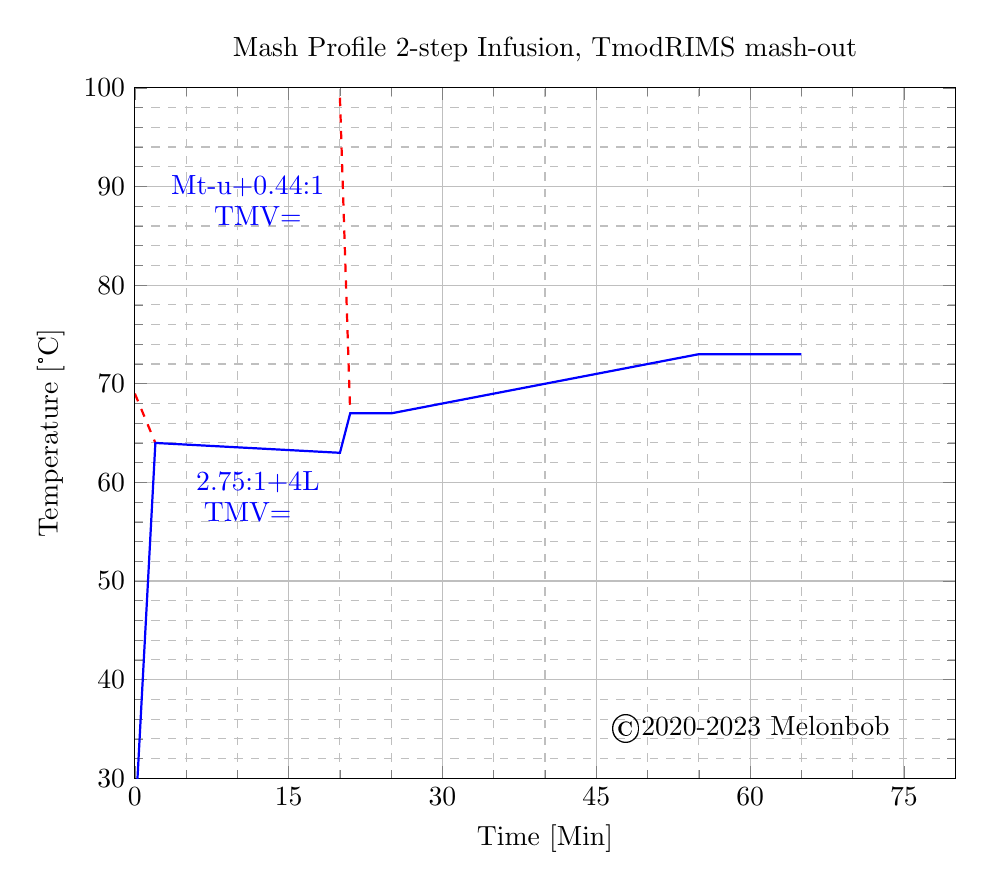
\begin{tikzpicture}
\begin{axis}[
    title={Mash Profile 2-step Infusion, TmodRIMS mash-out},
    xlabel={Time [Min]},
    ylabel={Temperature [\textdegree{C}]},
    xmin=0, xmax=80,
    ymin=30, ymax=100,
    xtick={0,15,30,45,60,75,90,105,120},
    ytick={30,40,50,60,70,80,90,100},
   % legend pos=north west,
    ymajorgrids=true,
    xmajorgrids=true,
    grid style=thin,
    %grid=major,
    minor grid style=dashed,
    yminorgrids=true,
    xminorgrids=true,
    yminorticks=true,
    xminorticks=true,
    minor y tick num=4,
    minor x tick num=2
]
\addplot [color=red,style=dashed,thick]
  coordinates {
    (0,69)% strike temp
    (2,64)% mash-in 2.75:1 (44+4L on PR1 w/ 16kg) TMV=48+0.67*16=59L
  };
\node [color=blue] at (axis cs:12,60) {2.75:1+4L};
\node [color=blue] at (axis cs:11,57) {TMV=};
\addplot [color=red, style=dashed,thick]
  coordinates {
    (20,99)(21,67)% 2INF 0.44:1 (7L on PR1 w/ 16 kg) TMV=66L
  };
\node [color=blue] at (axis cs:11,90) {Mt-u+0.44:1};
\node [color=blue] at (axis cs:12,87) {TMV=   };
\addplot [color=blue, style=thick]
  coordinates {
    (0,25)% initial grist temp
    (2,64)% mash-in, cooling loss w/o RIMS -4C/hr=-1C/15min
    (20,63)% beta rest 20'
    (21,67)% 2INF 0.44:1 7L on PR1
    (25,67)% saccharification alpha rest
    (55,73)% TmodRIMS 1C/5min
    (60,73)% 5' Lauter/ mash bed settle/ no RIMS
    (65,73)% 5' Vorlauf/ no hose
  };
% \legend{}
\node [color=black] at (axis cs:60,35) { \copyright 2020-2023 Melonbob };
 
\end{axis}
\end{tikzpicture}
\end{document}